In this chapter, we present the basics of \amrex.  The implementation
source codes are in {\tt amrex/Src/Base/}.  Note that \amrex\ classes
and functions are in namespace {\tt amrex}.  For clarity, we usually
drop {\tt amrex::} in the example codes here.  It is also assumed that
headers have been properly {\tt include}d.  We recommend you study
tutorials at {\tt amrex/Tutorials/Basic/} while reading this chapter.
After reading this chapter, one should be able to develop single-level
parallel codes using \amrex.  It should also be noted that this is not
a comprehensive reference manual.

\section{Dimensionality}
\label{sec:basics:dim}

As we have mentioned in Chapter~\ref{Chap:BuildingAMReX}, the
dimensionality of \amrex\ must be set at compile time.  A macro, {\tt
  AMREX\_SPACEDIM}, is defined to be the number of spatial
dimensions.  C++ codes can also use the {\tt amrex::SpaceDim}
variable.  Fortran codes can use either the macro and preprocessing or
do 
\begin{verbatim}
    use amrex_fort_module, only : amrex_spacedim
\end{verbatim}
The coordinate directions are zero based. \MarginPar{Not in Fortran}

\section{Array}

{\tt Array} class is derived from {\tt std::vector}.  The only
difference between {\tt Array} and {\tt std::vector} is that {\tt
  Array::operator[]} provides bound checking when compiled with {\tt
  DEBUG=TRUE}. 

\section{Real}

\amrex\ can be compiled to use either double precision (which is the
default) or single precision.  {\tt amrex::Real} is {\tt typedef}'d to
either {\tt double} or {\tt float}.  C codes can use {\tt
  amrex\_real}.  The data type is accessible in Fortran codes via
\begin{verbatim}
    use amrex_fort_module, only : amrex_real
\end{verbatim}

\section{ParallelDescriptor}

\amrex\ users do not need to use MPI directly.  Parallel communication
is often handled by the data abstraction classes (e.g., {\tt
  MultiFab}; Section~\ref{sec:basics:multifab}).  In addition, \amrex\
has provided {\tt namespace ParallelDesriptor}.  The frequently used
functions are 
\begin{lstlisting}[language=cpp]
 int myproc = ParallelDescriptor::MyProc();  // Return the rank
 
 int nprocs = ParallelDescriptor::NProcs();  // Return the number of processes
 
 if (ParallelDescriptor::IOProcessor()) { 
     // Only the I/O process executes this
 }
 
 int ioproc = ParallelDescriptor::IOProcessorNumber();  // I/O rank
 
 ParallelDescriptor::Barrier();
 
 // Broadcast 100 ints from the I/O Processor
 Array<int> a(100);
 ParallelDescriptor::Bcast(a.data(), a.size(),
                     ParallelDescriptor::IOProcessorNumber())
 
 // See AMReX_ParallelDescriptor.H for many other Reduce functions 
 ParallelDescriptor::ReduceRealSum(x);
\end{lstlisting}

\section{Print}
\label{sec:basics:print}

\amrex\ provides classes for printing messages to standard output or
any \cpp\ {\tt ostream}.  The main reason one should use them instead
of {\tt std::cout} is that messages from multiple processes or
threads do not get mixed up.  Below are some examples.
\begin{lstlisting}[language=cpp]
 Print() <<  "x = " << x << "\n"; // Print on I/O processor
 
 Real pi = std::atan(1.0)*4.0;
 // Print on rank 3 with precision of 17 digits
 // SetPrecision does not modify cout's floating-point decimal precision setting.
 Print(3).SetPrecision(17) << pi << "\n";

 int oldprec = std::cout.precision(10);
 Print() << pi << "\n";  // Print with 10 digits
 
 AllPrint() << "Every process prints\n";  // Print on every process
 
 std::ofstream ofs("my.txt", std::ofstream::out);
 Print(ofs) << "Print to a file" << std::endl;
 ofs.close();
\end{lstlisting}

\section{ParmParse}

{\tt ParmParse} is a class providing a database for the storage and
retrieval of command-line and input-file arguments.  When {\tt
  amrex::Initialize()} is called, the first command-line argument
after the executable name (if there is one and it does not contain
character {\tt =}) is taken to be the inputs file, and the contents in
the file are used to initialized the {\tt ParmParse} database.  The
rest of the command-line arguments are also parsed by {\tt ParmParse}.
The format of the inputs file is a series of definitions in the form
of {\tt prefix.name = value value ...}.  For each line, texts after a
{\tt \#} are comments.  Here is an example inputs file.
\begin{verbatim}
nsteps    = 100               # integer
nsteps    = 1000              # nsteps appears a second time
dt        = 0.03              # floating point number
ncells    = 128 64 32         # a list of 3 ints
xrange    = -0.5 0.5          # a list of 2 reals
title     = "Three Kingdoms"  # a string
hydro.cfl = 0.8               # with prefix, hydro 
\end{verbatim}
The following code shows how to use {\tt ParmParse} to get the values.
\begin{lstlisting}[language=cpp]
 ParmParse pp;
 
 int nsteps = 0;
 pp.query("nsteps", nsteps);
 amrex::Print() << nsteps << "\n";  // 1000
 
 Real dt;
 pp.get("dt", dt);  // runtime error if dt is not in inputs
 
 Array<int> numcells;
 // A different name say 'numcells' can be used
 pp.getarr("ncells", numcells);
 amrex::Print() << numcells.size() << "\n";  // 3
 
 Array<Real> xr {-1.0, 1.0};
 if (!queryarr("xrange", xr)) {
     amrex::Print() << "Cannot find xrange in inputs, "
                    << "so the default {-1.0,1.0} will be used\n";
 }
 
 std::string title;
 query("title", title);  // query string
 
 ParmParse pph("hydro");  // with prefix 'hydro'
 Real cfl;
 pph.get("cfl", cfl);    // get parameter with prefix
\end{lstlisting}
Note that when there are multiple definitions for a parameter {\tt
  ParamParse} by default returns the last one.  The difference between
{\tt query} and {\tt get} should also be noted.  It is a runtime error
if {\tt get} fails to get the value, whereas {\tt query} returns an
error code without generating a runtime error that will abort the run.
If it is sometimes convenient to override parameters with command-line
arguments without modifying the inputs file.  The command-line
arguments after the inputs file are added later to the database and
are therefore used be default.  For example, one can run with
\begin{verbatim}
    myexecutable myinputsfile ncells="64 32 16" hydro.cfl=0.9
\end{verbatim}
to change the value of {\tt ncells} and {\tt hydro.cfl}.

\section{Example of AMR Grids}
\label{sec:basics:amrgrids}

In block-structured AMR, there is a hierarchy of logically rectangular
grids.  The computational domain on each AMR level is decomposed into
a union of rectangular domains.  Figure~\ref{fig:basics:amrgrids} shows
an example of AMR grids.  There are three total levels in the example.
The coarsest grid ({\emph{black}) covers the domain with $16^2$
cells. Bold lines represent grid boundaries.  There are two
intermediate resolution grids ({\emph{blue}}) are at level 1 and the
cells are a factor of two finer than those at level 0.  The two
finest grids ({\emph{red}}) are at level 2 and the cells are a
factor of two finer than the level 1 cells.  Note that there is no
direct parent-child connection.  In this chapter, we will focus on
single levels.

\begin{figure}
  \centering
  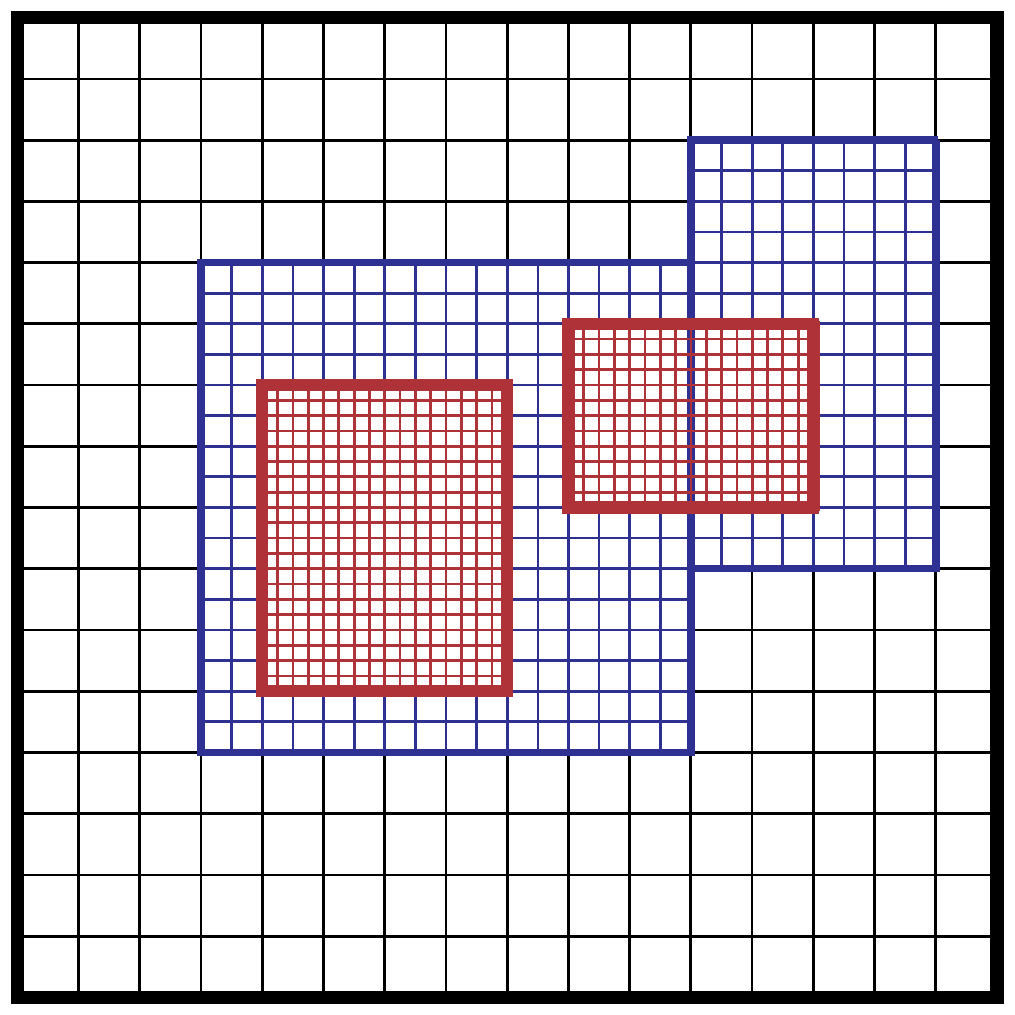
\includegraphics[width=3in]{./Basics/amrgrids.pdf}
  \caption{\label{fig:basics:amrgrids} Example of AMR grids.  There are
    three levels in total.}
\end{figure}

\section{Box, IntVect and IndexType}
\label{sec:basics:box}

{\tt Box} is the data structure for representing a rectangular domain
in indexing space.  For example, in Figure~\ref{fig:basics:amrgrids},
there are 1, 2 and 2 {\tt Box}es on levels 0, 1 and 2, respectively.
{\tt Box} is a dimension dependent class.  It has lower and upper
corners (represented by {\tt IntVect} and an index type (represented
by {\tt IndexType}).  There are no floating-point data in the object.

\subsection{IntVect}

{\idxamrex{IntVect}} is a dimension dependent class representing an
integer vector in {\idxamrex{AMREX\_SPACEDIM}}-dimensional space.  An
{\tt IntVect} can be constructed as follows,
\begin{lstlisting}[language=cpp]
 IntVect iv(AMREX_D_DECL(19, 0, 5));
\end{lstlisting}
Here {\tt AMREX\_D\_DECL} is a macro that expands {\tt
  AMREX\_D\_DECL(19,0,5)} to either {\tt 19} or {\tt 19,0} or {\tt
  19,0,5} depending on the number of dimensions.  The data can be
accessed via {\tt operator[]}, and the internal data pointer can be
returned by function {\tt getVect}.  For example
\begin{lstlisting}[language=cpp]
 for (int idim = 0; idim < AMREX_SPACEDIM; ++idim) {
     amrex::Print() << "iv[" << idim << "] = " << iv[idim] << "\n";
 }
 const int * p = iv.getVect();  // This can be passed to Fortran/C as an array
\end{lstlisting}

The class has a static function {\tt TheZeroVector()} returning the
zero vector, {\tt TheUnitVector()} returning the unit vector, and {\tt
  TheDimensionVector (int dir)} returning a reference to a constant
{\tt IntVect} that is zero except in the {\tt dir}-direction.  Note
the direction is zero-based.  {\tt IntVect} has a number of relational
operators, {\tt ==}, {\tt !=}, {\tt <}, {\tt <=}, {\tt >}, and {\tt
  >=} that can be used for lexicographical comparison (e.g., key of
{\tt std::map}), and a class {\tt IntVect::shift\_hasher} that can be
used as a hash function (e.g., for {\tt std::unordered\_map}).  It
also has various arithmetic operators.  For example,
\begin{lstlisting}[language=cpp]
 IntVect iv(AMREX_D_DECL(19, 0, 5));
 IntVect iv2((AMREX_D_DECL(4, 8, 0));
 iv += iv2;  // iv is now (23,8,5)
 iv *= 2;    // iv is now (46,16,10);
\end{lstlisting}

In AMR codes, one often needs to do refinement and coarsening on {\tt
  IntVect}.  The refinement operation can be done with the
multiplication operation.  However, the coarsening requires care
because of the rounding towards zero behavior of integer division in
Fortran, C and C++.  For example {\tt int i = -1/2} gives {\tt i =
  0}, and what we want is usually {\tt i = -1}.  Thus, one should use
the {\tt coarsen} functions:
\begin{lstlisting}[language=cpp]
  IntVect iv(AMREX_D_DECL(127,127,127));
  IntVect coarsening_ratio(AMREX_D_DECL(2,2,2));
  iv.coarsen(2);                 // Coarsen each component by 2
  iv.coarsen(coarsening_ratio);  // Component-wise coarsening
  const auto& iv2 = amrex::coarsen(iv, 2); // Return an IntVect w/o modifying iv
  IntVect iv3 = amrex::coarsen(iv, coarsening_return); // iv not modified
\end{lstlisting}

Finally, we note that {\tt operator<<} is overloaded for {\tt
  IntVect} and therefore one can call
\begin{lstlisting}[language=cpp]
  amrex::Print() << iv << "\n";
  std::cout << iv << "\n";
\end{lstlisting}

\subsection{IndexType}

This class defines an index as being cell based or node based in
each dimension.  The default constructor defines a cell based type in
all directions.  One can also construct an {\tt IndexType} with an
{\tt IntVect} with zero and one representing cell and node,
respectively.
\begin{lstlisting}[language=cpp]
 // Node in x-direction and cell based in y and z-directions
 // (i.e., x-face of numerical cells)
 IndexType xface(IntVect{AMREX_D_DECL(1,0,0)});
\end{lstlisting}
The class provides various functions including
\begin{lstlisting}[language=cpp]
 // True if the IndexType is cell based in all directions.
 bool cellCentered () const;

 // True if the IndexType is cell based in dir-direction.
 bool cellCentered (int dir) const;

 // True if the IndexType is node based in all directions.
 bool nodeCentered () const;

 // True if the IndexType is node based in dir-direction.
 bool nodeCentered (int dir) const;
\end{lstlisting}

Index type is a very important concept in \amrex.  It is a way of
representing the notion of indices $i$ and $i+1/2$.

\subsection{Box}

A {\tt Box} is an abstraction for defining discrete regions of {\tt
  AMREX\_SPACEDIM}-dimensional indexing space.  {\tt Box}es have an
{\tt IndexType} and two {\tt IntVect}s representing the lower and
upper corners.  Boxes can exist in positive and negative indexing
space.   Typical ways of defining a {\tt Box} are
\begin{lstlisting}[language=cpp]
 IntVect lo(AMREX_D_DECL(64,64,64));
 IntVect hi(AMREX_D_DECL(127,127,127));
 IndexType typ({AMREX_D_DECL(1,1,1)});
 Box cc(lo,hi);        // By default, Box is cell based.
 Box nd(lo,hi+1,typ);  // Construct a nodal Box.
 Print() << "A cell-centered Box " << cc << "\n";
 Print() << "An all nodal Box    " << nd << "\n";
\end{lstlisting}
Depending the dimensionality, the output of the code above is
\begin{verbatim}
  A cell-centered Box ((64,64,64) (127,127,127) (0,0,0))
  An all nodal Box    ((64,64,64) (128,128,128) (1,1,1))
\end{verbatim}
For simplicity, we will assume it is 3D for the rest of this section.
In the output, three integer tuples for each box are the lower corner
indices, upper corner indices, and the index types.  Note that {\tt 0}
and {\tt 1} denote cell and node, respectively.  For each tuple like
{\tt (64,64,64)}, the 3 numbers are for 3 directions.  The two {\tt
  Box}es in the code above represent different indexing views of the
same domain of $64^3$ cells.  Note that in \amrex\ convention, the
lower side of a cell has the same integer value as the cell centered
index.  That is if we consider a cell based index represent $i$, the
nodal index with the same integer value represents $i-1/2$.
Figure~\ref{fig:basics:indextypes} shows a 2D example of various index
types.  

\begin{figure}
  \centering
  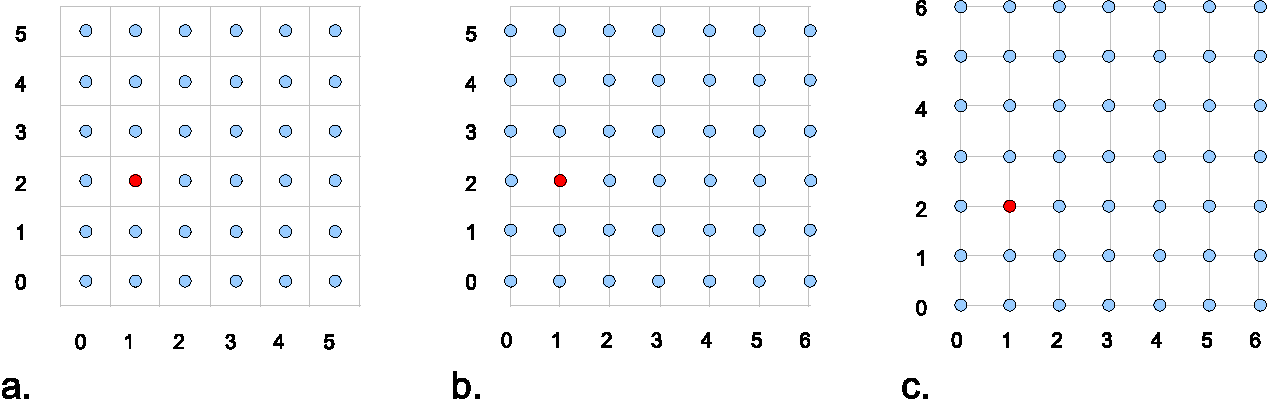
\includegraphics[width=5in]{./Basics/indextypes.pdf}
  \caption{\label{fig:basics:indextypes} Some of the different index
    types in two dimensions: (a) cell-centered, (b) face-centered,
    i.e., nodal in one dimensions ($x$) only, and (c) corner/nodal,
    i.e., nodal in all dimensions.  Note that for data that is nodal
    in one or more direction, the integer index corresponds to the
    lower boundary in that direction.}
\end{figure}

There are a number of ways of converting a {\tt Box} from one type to
another.
\begin{lstlisting}[language=cpp]
  Box b0 ({64,64,64}, {127,127}); // Index type: (cell, cell, cell)

  Box b1 = surroundingNodes(b0);  // A new Box with type (node, node, node)
  Print() << b1;                  // ((64,64,64) (128,128,128) (1,1,1))
  Print() << b0;                  // Still ((64,64,64) (127,127,127) (0,0,0))

  Box b2 = enclosedCells(b1);     // A new Box with type (node, node, node)
  if (b2 == b0) {                 // Yes, they are identical.
     Print() << "b0 and b2 are identical!\n";
  }

  Box b3 = convert(b0, {0,1,0});  // A new Box with type (cell, node, cell)
  Print() << b3;                  // ((64,64,64) (127,128,127) (0,1,0))

  b3.convert({0,0,1});            // Convert b0 to type (cell, cell, node)
  Print() << b3;                  // ((64,64,64) (127,127,128) (0,0,1))

  b3.surroundingNodes();          //  Exercise for you
  b3.enclosedCells();             //  Exercise for you
\end{lstlisting}

The internal data of {\tt Box} can be accessed via various member functions.
Examples are
\begin{lstlisting}[language=cpp]
  const IntVect& smallEnd () const&;  // Get the small end of the Box
  int bigEnd (int dir) const;         // Get the big end in dir direction
  const int* loVect () const&;        // Get a const pointer to the lower end
  const int* hiVect () const&;        // Get a const pointer to the upper end
\end{lstlisting}

{\tt Box}es can be refined and coarsened.  Refinement or coarsening
does not change the index type.  Some examples are shown below.
\begin{lstlisting}[language=cpp]
  Box ccbx ({16,16,16}, {31,31,31});
  ccbx.refine(2);
  Print() << ccbx;                   // ((32,32,32) (63,63,63) (0,0,0))
  Print() << ccbx.coarsen(2);        // ((16,16,16) (31,31,31) (0,0,0))

  Box ndbx ({16,16,16}, {32,32,32}, {1,1,1});
  ndbx.refine(2);
  Print() << ndbx;                   // ((32,32,32) (64,64,64) (1,1,1))
  Print() << ndbx.coarsen(2);        // ((16,16,16) (32,32,32) (1,1,1))

  Box facebx ({16,16,16}, {32,31,31}, {1,0,0});
  facebx.refine(2);
  Print() << facebx;                 // ((32,32,32) (64,63,63) (1,0,0))
  Print() << facebx.coarsen(2);      // ((16,16,16) (32,31,31) (1,0,0))

  Box uncoarsenable ({16,16,16}, {30,30,30});
  print() << uncoarsenable.coarsen(2); // ({8,8,8}, {15,15,15});
  print() << uncoarsenable.refine(2);  // ({16,16,16}, {31,31,31});
                                       // Different from the original!
\end{lstlisting}
Note that refinement and coarsening behaviors depend on the indexing
type.  One should think the refinement and coarsening in AMR context
that refined or coarsened {\tt Box} still covers the same physical
domain.  {\tt Box uncoarsenable} in the example above is considered
uncoarsenable because its coarsened version does not cover the same
physical domain in the AMR context.

{\tt Box}es can grow and they can grow in all directions or just one
direction.  There are a number of {\tt grow} functions.  Some are
member functions of the {\tt Box} class and others are non-member
functions in the {\tt amrex} namespace. 

{\tt Box} class provides the following member functions testing if a {\tt
  Box} or {\tt IntVect} is contained within this {\tt Box}.  Note that
it is a runtime error if the two {\tt Box}es have different types.
\begin{lstlisting}[language=cpp]
  bool contains (const Box& b) const;
  bool strictly_contains (const Box& b) const;
  bool contains (const IntVect& p) const;
  bool strictly_contains (const IntVect& p) const;
\end{lstlisting}

Another very common operation is the intersection of two {\tt Box}es
like in the following examples.
\begin{lstlisting}[language=cpp]
  Box b0 ({16,16,16}, {31,31,31});
  Box b1 ({ 0, 0,30}, {23,23,63});
  if (b0.intersects(b1)) {                  // true
      Print() << "b0 and b1 intersect.\n"; 
  }

  Box b2 = b0 & b1;     // b0 and b1 unchanged
  Print() << b2;        // ((16,16,30) (23,23,31) (0,0,0))

  Box b3 = surroundingNodes(b0) & surroundingNodes(b1); // b0 and b1 unchanged
  Print() << b3;        // ((16,16,30) (24,24,32) (1,1,1))

  b0 &= b2;             // b2 unchanged
  Print() << b0;        // ((16,16,30) (23,23,31) (0,0,0))

  b0 &= b3;             // Runtime error because of type mismatch!
\end{lstlisting}

\section{RealBox and Geometry}

A {\tt RealBox} stores the physical location in floating-point numbers
of the lower and upper corners of a rectangular domain.

{\tt Geometry} class describes problem domain and coordinate system
for rectangular problem domains.  A {\tt Geometry} object can be
constructed with
\begin{lstlisting}[language=cpp]
  explicit Geometry (const Box&     dom,
                     const RealBox* rb     = nullptr,
                     int            coord  = -1,
                     int*           is_per = nullptr);
\end{lstlisting}
Here the constructor takes a {\tt Box} specifying the indexing space
domain, an optional argument of {\tt RealBox} pointer specifying the
physical domain, an optional {\tt int} specifying coordinate system
type, and an optional {\tt int *} specifying periodicity.  If a {\tt
  RealBox} is not given, \amrex\ will construct one based on {\tt
  ParmParse} parameters, {\tt geometry.prob\_lo} and {\tt
  geometry.prob\_hi}, where each of the parameter is an array of {\tt
  AMREX\_SPACEDIM} real numbers.  It's a runtime error if this fails.
The optional argument for coordinate system is an integer type with
valid values being 0 (Cartesian), or 1 (cylindrical), or 2
(spherical).  If it is invalid as in the case of the default argument
value, \amrex\ will query the {\tt ParmParse} database for {\tt
  geometry.coord\_sys} and use it if one is found.  If it cannot find
the parameter, the coordinate system is set to 0 (i.e., Cartesian
coordinates).  {\tt Geometry} class has the concept of periodicity.
An optional argument can be passed specifying periodicity in each
dimension.  If it is not given, the domain is assumed to be
non-periodic unless there is the {\tt ParmParse} integer array
parameter {\tt geometry.is\_periodic} with {\tt 0} denoting
non-periodic and {\tt 1} denoting periodic.  Below is an example of
defining a {\tt Geometry} for a periodic rectangular domain of
$[-1.0,1.0]$ in each direction discretized with $64$ numerical cells
in each direction.
\begin{lstlisting}[language=cpp]
  int n_cell = 64;

  // This defines a Box with n_cell cells in each direction.
  Box domain(IntVect{AMREX_D_DECL(       0,        0,        0)},
             IntVect{AMREX_D_DECL(n_cell-1, n_cell-1, n_cell-1)});

  // This defines the physical box, [-1,1] in each direction.
  RealBox real_box({AMREX_D_DECL(-1.0,-1.0,-1.0)},
                   {AMREX_D_DECL( 1.0, 1.0, 1.0)});
  
  // This says we are using Cartesian coordinates
  int coord = 0;
  
  // This sets the boundary conditions to be doubly or triply periodic
  std::array<int,AMREX_SPACEDIM> is_periodic {AMREX_D_DECL(1,1,1)};
  
  // This defines a Geometry object
  Geometry geom(domain, &real_box, coord, is_periodic.data());
\end{lstlisting}

A {\tt Geometry} object can return various information of the physical
domain and the indexing space domain.  For example,
\begin{lstlisting}[language=cpp]
  const Real* problo = geom.ProbLo();  // Lower corner of the physical domain
  Real yhi = geom.ProbHi(1);           // y-direction upper corner
  const Real* dx = geom.CellSize();    // Cell size for each direction
  const Box& domain = geom.Domain();   // Index domain
  bool is_per = geom.isPeriodic(0);    // Is periodic in x-direction?
\end{lstlisting}


\section{BoxArray}
\label{sec:basics:ba}

{\tt BoxArray} is a class for storing a collection of {\tt Box}es on
a single AMR level.  One can make a {\tt BoxArray} out of a single {\tt Box}
and then chop it into multiple {\tt Box}es.
\begin{lstlisting}[language=cpp]
  Box domain(IntVect{0,0,0}, IntVect{127,127,127});
  BoxArray ba(domain);  // Make a new BoxArray out of a single Box
  Print() << "BoxArray size is " << ba.size() << "\n";  // 1
  ba.maxSize(64);       // Chop into boxes of 64^3 cells
  Print() << ba;
\end{lstlisting}
The output is like below,
\begin{verbatim}
  (BoxArray maxbox(8)
         m_ref->m_hash_sig(0)
  ((0,0,0) (63,63,63) (0,0,0)) ((64,0,0) (127,63,63) (0,0,0))
  ((0,64,0) (63,127,63) (0,0,0)) ((64,64,0) (127,127,63) (0,0,0))
  ((0,0,64) (63,63,127) (0,0,0)) ((64,0,64) (127,63,127) (0,0,0))
  ((0,64,64) (63,127,127) (0,0,0)) ((64,64,64) (127,127,127) (0,0,0)) )
\end{verbatim}
It shows that {\tt ba} now has 8 {\tt Box}es, and it also prints out
each {\tt Box}es.  

In \amrex, {\tt BoxArray} is a global data structure.  It holds all
the {\tt Box}es in a collection, even though a single process in a
parallel run only owns some of the {\tt Box}es via domain
decomposition.  In the example above, a 4-process run may divide the
work and each process owns say 2 {\tt Box}es
(Section~\ref{sec:basics:dm}).  Each process can then allocate memory
for the floating point data on the {\tt Box}es it owns
(Sections~\ref{sec:basics:multifab} \& \ref{sec:basics:fab}). 

{\tt BoxArray} has an indexing type, just like {\tt Box}.  Each {\tt
  Box} in a {\tt BoxArray} has the same type as the {\tt BoxArray}
itself.  In the following example, we show how one can convert {\tt
  BoxArray} to a different type. 
\begin{lstlisting}[language=cpp]
  BoxArray cellba(Box(IntVect{0,0,0}, IntVect{63,127,127}));
  cellba.maxSize(64);
  BoxArray faceba = cellba;
  // convert to index type (cell, cell, node)
  faceba.convert(IntVect{0,0,1});
  // Return an all node BoxArray
  const BoxArray& nodeba = amrex::convert(faceba, IntVect{1,1,1});
  Print() << cellba[0] << "\n";  // ((0,0,0) (63,63,63) (0,0,0))
  Print() << faceba[0] << "\n";  // ((0,0,0) (63,63,64) (0,0,1))  
  Print() << nodeba[0] << "\n";  // ((0,0,0) (64,64,64) (1,1,1))
\end{lstlisting}

As shown in the example above, {\tt BoxArray} has an {\tt operator[]}
that returns a {\tt Box} given an index.  It should be emphasized that
there is a difference between its behavior and the usual behavior of
an subscript operator one might expect.  The subscript operator in
{\tt BoxArray} returns by value instead of reference.  This means code
like below is meaningless because it modifies a temporary return
value. 
\begin{lstlisting}[language=cpp]
  ba[3].coarsen(2);  // DO NOT DO THIS!  Doesn't do what one might expect.
\end{lstlisting}

{\tt BoxArray} has a number of member functions that allow the {\tt
  Box}es to be modified.  For example,
\begin{lstlisting}[language=cpp]
  BoxArray& refine (int refinement_ratio);   // Refine each Box in BoxArray
  BoxArray& refine (const IntVect& refinement_ratio);
  BoxArray& coarsen (int refinement_ratio);  // Coarsen each Box in BoxArray
  BoxArray& coarsen (const IntVect& refinement_ratio);
\end{lstlisting}

We have mentioned at the beginning of this section that {\tt BoxArray}
is a global data structure storing {\tt Box}es owned by all processes.
The operation of deep copy is thus undesirable because the operation
itself is expensive and the extra copy wastes memory.  The
implementation of the {\tt BoxArray} class uses {\tt std::shared\_ptr}
to an internal container holding the actual {\tt Box} data.  Thus
making a copy of {\tt BoxArray} is a quite cheap operation.  The
conversion of types and coarsening are also cheap because they can
share the internal data with the original {\tt BoxArray}.  Function
{\tt refine} does create a new deep copy of the original data.  Also
note that a {\tt BoxArray} and its variant with a different type share
the same internal data is an implementation detail.  We discuss this
so that the users are aware of the performance and resource cost.
Conceptually we can think of them as completely independent of each
other.

For advanced users, \amrex\ provides functions performing the
intersection of a {\tt BoxArray} and a {\tt Box}.  These functions are
much faster than a naive implementation of performing intersection of
the {\tt Box} with each {\tt Box} in the {\tt BoxArray}.  If one needs
to perform those intersections, functions {\tt amrex::intersect}, {\tt
  BoxArray:: intersects} and {\tt BoxArray::intersections} should be
used.

\section{DistributionMapping}
\label{sec:basics:dm}

{\tt DistributionMapping} is a class describes which process owns the
data living on the domains specified by the {\tt Box}es in a {\tt
  BoxArray}.  Like {\tt BoxArray}, {\tt DistributionMapping} has an
element for each {\tt Box}, including the ones owned by other parallel
processes.  A way to construct a {\tt DistributionMapping} object
given a {\tt BoxArray} is as follows.
\begin{lstlisting}[language=cpp]
  DistributionMapping dm {ba};
\end{lstlisting}
Oftentimes what one needs is simply making a copy. 
\begin{lstlisting}[language=cpp]
  DistributionMapping dm {another_dm};
\end{lstlisting}
Note that this class is built using {\tt std::shared\_ptr}.  Thus
making a copy is relatively cheap in terms of performance and memory
resources.  This class has a subscript operator that returns the
process ID at a given index.

By default, {\tt DistributionMapping} uses an algorithm based on space
filling curve to determine distribution.  One can change the default
via {\tt ParmParse} paramter {\tt DistributionMapping.strategy}.  {\tt
  KNAPSACK} is a common choice that is optimized for load balance.
One can also explicitly construct a certain type of distribution.
{\tt DistributionMapping} class allows the user to have complete control by
passing an array of integers. 
\begin{lstlisting}[language=cpp]
  DistributionMapping dm;   // empty object
  Array<int> pmap;
  // The user fills the pmap array with the values specifying owner processes
  dm.define(pmap);  // Build DistributionMapping given an array of process IDs.
\end{lstlisting}


\section{BaseFab, FArrayBox and IArrayBox}
\label{sec:basics:fab}

\amrex\ is a block-structured AMR framework.  Although AMR introduces
irregularity to the data and algorithms, there is regularity at the
block/{\tt Box} level due to rectangular domain and the data structure
at the {\tt Box} level is conceptually simple.  {\tt BaseFab} is a
class template for multi-dimensional array-like data structure on a
{\tt Box}.  The template parameter is typically basic types such as
{\tt Real}, {\tt int} or {\tt char}.  The dimensionality of the array
is {\tt AMREX\_SPACEDIM} plus one.  The additional dimensional is for
the number of components.  The data are internally stored in a
contiguous block of memory in Fortran array order (i.e., column-major
order) for $(x,y,z,\mathrm{component})$, and each component also
occupies a contiguous block of memory because of the ordering.  For
example, a {\tt BaseFab<Real>} with 4 components defined on a
three-dimensional {\tt Box(IntVect\{-4,8,32\},IntVect\{32,64,48\})} is
like a Fortran array of {\tt real(amrex\_real),
  dimension(-4:32,8:64,32:48,0:3)}.  Note that the convention in \cpp\
part of \amrex\ is the component index is zero based.  The code for
constructing such an object is as follows,
\begin{lstlisting}[language=cpp]
  Box bx(IntVect{-4,8,32}, IntVect{32,64,48});
  int numcomps = 4;
  BaseFab<Real> fab(bx,numcomps);
\end{lstlisting}

Most applications do not use {\tt BaseFab} directly, but utilize
specialized classes derived from {\tt BaseFab}.  The most common types
are {\tt FArrayBox} derived from {\tt BaseFab<Real>} and {\tt
  IArrayBox} derived from {\tt BaseFab<int>}.

These derived classes also obtain many {\tt BaseFab} member functions
via inheritance.  We now show some common usages of these functions.
To get the {\tt Box} where a {\tt BaseFab} or its derived object is
defined, one can call
\begin{lstlisting}[language=cpp]
  const Box& box() const;
\end{lstlisting}
To the number of component, one can call
\begin{lstlisting}[language=cpp]
  int nComp() const;
\end{lstlisting}
To get a pointer to the array data, one can call
\begin{lstlisting}[language=cpp]
  T* dataPtr(int n=0);     // Data pointer to the nth component
                           // T is template parameter (e.g., Real)
  const T* dataPtr(int n=0) const; // const version
\end{lstlisting}
The typical usage of the returned pointer is then to pass it to a
Fortran or C function that works on the array data (see
Section~\ref{sec:basics:fortran}).
{\tt BaseFab} has several functions that set the array data to a
constant value (e.g., 0).  Two examples are as follows.  
\begin{lstlisting}[language=cpp]
  void setVal(T x);        // Set all data to x
  // Set the sub-region specified by bx to value x starting from component
  // nstart.  ncomp is the total number of component to be set.
  void setVal(T x, const Box& bx, int nstart, int ncomp);
\end{lstlisting}
One can copy data from one {\tt BaseFab} to another.
\begin{lstlisting}[language=cpp]
  BaseFab<T>& copy (const BaseFab<T>& src, const Box& srcbox, int srccomp,
                    const Box& destbox, int destcomp, int numcomp);
\end{lstlisting}
Here the function copies the data from the region specified by {\tt
  srcbox} in the source {\tt BaseFab src} into the region specified by
{\tt destbox} in the destination {\tt BaseFab} that invokes the
function.  Note that although {\tt srcbox} and {\tt destbox} may be
different, they must be the same size and shape, otherwise a runtime
error occurs.  The user also specifies how many components ({\tt int
  numcomp}) are copied starting at component {\tt srccomp} in {\tt
  src} and stored starting at component {\tt destcomp}.  {\tt BaseFab}
has functions returning the minimum or maximum value.
\begin{lstlisting}[language=cpp] 
  T min (int comp=0) const;  // Minimum value of given component.
  T min (const Box& subbox, int comp=0) const; // Minimum value of given 
                                               // component in given subbox.
  T max (int comp=0) const;  // Maximum value of given component.
  T max (const Box& subbox, int comp=0) const; // Maximum value of given 
                                               // component in given subbox.
\end{lstlisting}

{\tt BaseFab} also has many arithmetic functions.  Here are some
examples using {\tt FArrayBox}.
\begin{lstlisting}[language=cpp]
  Box box(IntVect{0,0,0}, IntVect{63,63,63});
  int ncomp = 2;
  FArrayBox fab1(box, ncomp);
  FArrayBox fab2(box, ncomp);
  fab1.setVal(1.0);    // Fill fab1 with 1.0
  fab1.mult(10.0, 0);  // Multiply component 0 by 10.0
  fab2.setVal(2.0);    // Fill fab2 with 2.0
  Real a = 3.0;
  fab2.saxpy(a, fab1); // For both components, fab2 <- a * fab1 + fab2
\end{lstlisting}
For more complicated expressions that not supported, one can write
Fortran or C functions for those (Section~\ref{sec:basics:fortran}).
Note that {\tt BaseFab} does provide operators for accessing the
data directly in \cpp.  For example, the {\tt saxpy} example above can
be done with
\begin{lstlisting}[language=cpp]
  // Iterate over all components
  for (int icomp=0; icomp < fab1.nComp(); ++icomp) {
      // Iterate over all cells in Box
      for (BoxIterator bit(fab1.box()); bit.ok(); ++bit) {
          // bit() returns IntVect
          fab2(bit(),icomp) = a * fab1(bit(),icomp) + fab2(bit(),icomp);
      }
  }
\end{lstlisting}
But this approach is generally not recommended for performance reason.
However, it can be handy for debugging.

{\tt BaseFab} and its derived classes are containers data on {\tt
  Box}.  We recall that {\tt Box} has types
(Section~\ref{sec:basics:box}).  The examples in this section so far
use the default cell based type.  However, some functions will result
in a runtime error if the types mismatch.  For example.
\begin{lstlisting}[language=cpp]
  Box ccbx ({16,16,16}, {31,31,31});           // cell centered box
  Box ndbx ({16,16,16}, {31,31,31}, {1,1,1});  // nodal box
  FArrayBox ccfab(ccbx);
  FArrayBox ndfab(ndbx);
  ccfab.setVal(0.0);
  ndfab.copy(ccfab);   // runtime error due to type mismatch
\end{lstlisting}

Because it typically contains a lot of data, {\tt BaseFab}'s copy
constructor and copy assignment operator are disabled for performance
reason.  However, it does provide a move constructor.  In addition, it
also provides a constructor for making an alias of an existing
object.  Here is an example using {\tt FArrayBox}.
\begin{lstlisting}[language=cpp]
  FArrayBox orig_fab(box, 4);  // 4-component FArrayBox
  // Make a 2-component FArrayBox that is an alias of rhs
  // starting from component 1.
  FArrayBox alias_fab(rhs, amrex::make_alias, 1, 2);
\end{lstlisting}
In the example, the alias {\tt FArrayBox} has only two components even
though the original one has four components.  The alias has a sliced
component view of the original {\tt FArrayBox}.  This is possible
because of the array ordering.  It is however not possible to slice in
the real space (i.e., the first {\tt AMREX\_SPACEDIM} dimensions).
Note that no new memory is allocated in constructing the alias and the
alias contains a non-owning pointer.  It should be emphasized that the
alias will contain a dangling pointer after the original {\tt
  FArrayBox} reaches its end of life.

\section{FabArray, MultiFab and iMultiFab}
\label{sec:basics:multifab}

{\tt FabArray<FAB>} is a class template for a collection of {\tt FAB}s
on the same AMR level associated with a {\tt BoxArray}
(Section~\ref{sec:basics:ba}).  The template parameter {\tt FAB} is
usually {\tt BaseFab<T>} or its derived classes (e.g., {\tt
  FArrayBox}).  However, it can also be used to hold other data
structures.  To construct a {\tt FabArray}, a {\tt BoxArray} must be
provided because it is intended to hold {\emph{grid}} data defined on
a union of rectangular regions embedded in a uniform index space.  For
example, an {\tt FabArray} object can be used to hold data for one
level of the example grids of Figure~\ref{fig:basics:amrgrids}.  The
{\tt BoxArray} on level 2 ({\emph{red}) has two {\tt Box}es.

{\tt FabArray} is a parallel data structure that the data (i.e.,
{\tt FAB}) are distributed among parallel processes.  On each process,
the {\tt FabArray} contains only the {\tt FAB} objects owned by this
process, and the process operates only on its local data.  For
operations that require data owned by other processes, remote
communications are involved.  Thus, the construction of a {\tt
  FabArray} requires a {\tt DistributionMapping}
(Section~\ref{sec:basics:dm}) that specifies which process owns which
{\tt Box}.  For level 2 ({\emph{red}) in
Figure~\ref{fig:basics:amrgrids}, there are two {\tt Box}es.  Suppose
there are two parallel processes, and we use a {\tt
  DistributionMapping} that assigns one {\tt Box} to each process.
For {\tt FabArray} on each process, it is built on a {\tt BoxArray} with
2 {\tt Box}es, but contains only one {\tt FAB}.  

In \amrex, there are some specialized classes derived from {\tt
  FabArray}.  The {\tt iMultiFab} class is derived from {\tt
  FabArray<IArrayBox>}.  The most commonly used {\tt FabArray} kind
class is {\tt MultiFab} derived from {\tt FabArray<FArrayBox>}.  In
the rest of this section, we use {\tt MultiFab} as example.  However,
these concepts are equally applicable to other types of {\tt
  FabArray}s.  There are many ways to define a {\tt MultiFab}.  For
example,
\begin{lstlisting}[language=cpp]
  // ba is BoxArray
  // dm is DistributionMapping
  int ncomp = 4;
  int ngrow = 1;
  MultiFab mf(ba, mf, ncomp, ngrow);
\end{lstlisting}
Here we define a {\tt MultiFab} with 4 components and 1 ghost cell.  A
{\tt MultiFab} contains a number of {\tt FArrayBox}es
(Section~\ref{sec:basics:fab}) defined on {\tt Box}es grown by the
number of ghost cells (1 in this example).  That is the {\tt Box} in
the {\tt FArrayBox} is not exactly the same as in the {\tt BoxArray}.
If the {\tt BoxArray} has a {\tt Box\{(8,8,8) (15,15,15)\}}, the one
used for constructing {\tt FArrayBox} will be {\tt Box\{(7,7,7)
  (16,16,16)\}} in this example.  For cells in {\tt FArrayBox}, we
call those in the original {\tt Box} valid cells and the grown part
ghost cells.  Note that {\tt FArrayBox} itself alone does not have the
concept of ghost cell, whereas ghost cell is a key concept of {\tt
  MultiFab} that allows for local operations on ghost cell data
originated from remote processes.  We will discuss how to fill ghost
cells with data from valid cells later in this section.  {\tt
  MultiFab} also has a default constructor.  One can define an empty
{\tt MultiFab} first and then call the {\tt define} function as
follows.
\begin{lstlisting}[language=cpp]
  MultiFab mf;
  // ba is BoxArray
  // dm is DistributionMapping
  int ncomp = 4;
  int ngrow = 1;
  mf.define(ba, mf, ncomp, ngrow);
\end{lstlisting}
Given an existing {\tt MultiFab}, one can also make an alias {\tt
  MultiFab} as follows.
\begin{lstlisting}[language=cpp]
  // orig_mf is an existing Multifab
  int start_comp = 3;
  int num_comps = 1;
  MultiFab alias_mf(orig_mf, amrex::make_alias, start_comp, num_comps);
\end{lstlisting}
Here the first integer parameter is the starting component in the
original {\tt MultiFab} that will become component 0 in the alias {\tt
  MultiFab} and the second integer parameter is the number of
components in the alias.  It's a runtime error if the sum of the two
integer parameters is greater than the number of the components in the
original {\tt MultiFab}.  Note that the alias {\tt MultiFab} has
exactly the same number of ghost cells as the original {\tt MultiFab}.

We often need to build new {\tt MultiFab}s that have the same {\tt
  BoxArray} and {\tt DistributionMapping} as a given {\tt MultiFab}.
Below is an example of how to achieve this.
\begin{lstlisting}[language=cpp]
  // mf0 is an already defined MultiFab
  const BoxArray& ba = mf0.boxArray();
  const DistributionMapping& dm = mf0.DistributionMap();
  int ncomp = mf0.nComp();
  int ngrow = mf0.ngrow();
  MultiFab mf1(ba,dm,ncomp,ngrow);  // new MF with the same ncomp and ngrow
  MultiFab mf2(ba,dm,ncomp,0);      // new MF with no ghost cells
  // new MF with 1 component and 2 ghost cells
  MultiFab mf3(mf0.boxArray(), mf0.DistributionMap(), 1, 2);               
\end{lstlisting}

As we have repeatedly mentioned in this chapter that {\tt Box} and
{\tt BoxArray} have various index types.  Thus, {\tt MultiFab} also
has an index type that is obtained from the {\tt BoxArray} used for
defining the {\tt MultiFab}.  It should be noted again that index type
is a very important concept in \amrex.  Let's consider an example of a
finite-volume code, in which the state is defined as cell averaged
variables and the fluxes are defined as face averaged variables.
\begin{lstlisting}[language=cpp]
  // ba is cell-centered BoxArray
  // dm is DistributionMap
  int ncomp = 3;  // Suppose the system has 3 components
  int ngrow = 0;  // no ghost cells
  MultiFab state(ba, dm, ncomp, ngrow);
  MultiFab xflux(amrex::convert(ba, IntVect{1,0,0}), dm, ncomp, 0);
  MultiFab yflux(amrex::convert(ba, IntVect{0,1,0}), dm, ncomp, 0);
  MultiFab zflux(amrex::convert(ba, IntVect{0,0,1}), dm, ncomp, 0);
\end{lstlisting}
Here all {\tt MultiFab} use the same {\tt DistributionMapping}, but
their {\tt BoxArray}s have different.  The state is cell based,
whereas the fluxes are on the faces.  Suppose the cell based {\tt
  BoxArray} contains a {\tt Box\{(8,8,16), (15,15,31)\}}.  The state
on that {\tt Box} is conceptually a Fortran Array with the dimension
of {\tt (8:15,8:15,16:31,0:2)}.  The fluxes are arrays with slightly
different indices.  For example, the $x$-direction flux for that {\tt
  Box} has the dimension of {\tt (8:16,8:15,16:31,0:2)}.  Note there is
an extra element in $x$-direction.  

The {\tt MultiFab} provides many functions performing common
arithmetic operations on a {\tt MultiFab} or between {\tt MultiFab}s
built with the {\emph{same}} {\tt BoxArray} and {\tt DistributionMap}.
For example,
\begin{lstlisting}[language=cpp]
  Real dmin = mf.min(3);   // Minimum value in component 3 of MultiFab mf
                           // no ghost cells included
  Real dmax = mf.max(3,1); // Maximum value in component 3 of MultiFab mf
                           // including 1 ghost cell
  mf.setVal(0.0);          // Set all values to zero including ghost cells

  MultiFab::Add(mfdst, mfsrc, sc, dc, nc, ng);  // Add mfsrc to mfdst
  MultiFab::Copy(mfdst, mfsrc, sc, dc, nc, ng); // Copy from mfsrc to mfdst
  // MultiFab mfdst: destination 
  // MultiFab mfsrc: source
  // int      sc   : starting component index in mfsrc for this operation
  // int      dc   : starting component index in mfdst for this operation
  // int      sc   : number of components for this operation
  // int      ng   : number of ghost cells involved in this operation
\end{lstlisting}
We refer the reader to {\tt Src/Base/AMReX\_MultiFab.H} and {\tt
  Src/Base/AMReX\_FabArray.H} for more details.  It should be noted
again it is a runtime error if the two {\tt MultiFab}s passed to functions
like {\tt MultiFab::Copy} are not built with the {\emph{same}} {\tt
  BoxArray} (including index type) and {\tt DistributionMap}. 

It is usually the case that the {\tt Box}es in the {\tt BoxArray} used
for building a {\tt MultiFab} are non-intersecting except that they
can be overlapping due to nodal index type.  However, {\tt MultiFab}
can have ghost cells, and in that case {\tt FArrayBox}es are defined
on {\tt Box}es larger than the {\tt Box}es in the {\tt BoxArray}.
Parallel communication is then needed to fill the ghost cells with
valid cell data from other {\tt FArrayBox}es possibly on other
parallel processes.  The function for performing this type of
communication is {\tt FillBoundary}.
\begin{lstlisting}[language=cpp]
  MultiFab mf(...parameters omitted...);
  Geometry geom(...parameters omitted...);
  mf.FillBoundary();                    // Fill ghost cells for all components
                                        // Periodic boundaries are not filled.
  mf.FillBoundary(geom.periodicity());  // Fill ghost cells for all components
                                        // Periodic boundaries are not filled.
  mf.FillBoundary(2, 3);        // Fill 3 components starting from component 2
  mf.FillBoundary(geom.periodicity(), 2, 3);
\end{lstlisting}
Note that {\tt FillBoundary} does not modify any valid cells.  Also
note that {\tt MultiFab} itself does not have the concept of
periodicity boundary, but {\tt Geometry} has, and we can provide that
information so that periodic boundaries can be filled as well.

% parallel communication copy

\section{MFIter and Tiling}
\label{sec:basics:mfiter}

\section{Calling Fortan or C}
\label{sec:basics:fortran}

\section{Physical Boundary}

\section{I/O}

\section{Memory Allocation}

% resize

\section{Abort, Assertion, Floating-Point Exceptions, and Backtrace}
% FArrayBox init nan check nan .... contains_nan
